\documentclass[final]{beamer}
\usetheme{Madrid}

%%%%%%%%%%%%%%% PACKAGES %%%%%%%%%%%%%%%%%%%%%%%
\usepackage{bm}                 % for bold symbols - allows use of \bm

%% The algorithm defines the algorithm floating environment and the algpseudocode package is useful for constructing Pseudo code.
\usepackage{algorithm}
\usepackage{algpseudocode}
\algnewcommand{\IIf}[1]{\State\algorithmicif #1\ \algorithmicthen}
\algnewcommand{\EndIIf}{\unskip}

%% For creating pictures
\usepackage{tikz}
\usetikzlibrary{calc}
%\usepackage{pgfplotstable}
\usepackage{pgfplots}
%\pgfplotsset{compat=newest}
%         every axis plot post/.append style={green,mark=none}}

%% For making algorithms float
\usepackage{float}
\newfloat{algorithm}{t}{lop}
%% For creating draft watermark
%\usepackage{draftwatermark}
%\SetWatermarkText{DRAFT}
%\SetWatermarkScale{1}

\usepackage{amsmath}            % for split environment
%\newtheorem{example}{Example}

\usepackage{bbm}                % for indicator function

\usepackage{pdfpages}           % For including pdfs

%% Declaring \argmin and \argmax operators:
\DeclareMathOperator*{\argmin}{arg\,min}
\DeclareMathOperator*{\argmax}{arg\,max}
%% Declare trace operator \Tr:
\DeclareMathOperator*{\Tr}{Tr}
%% Declare pdf functions
\DeclareMathOperator*{\Cat}{Cat}
\DeclareMathOperator*{\Dir}{Dir}
\DeclareMathOperator*{\DP}{DP}
\DeclareMathOperator*{\BetaDist}{Beta}
\DeclareMathOperator*{\GammaDist}{Gamma}
\DeclareMathOperator*{\GEM}{GEM}
\DeclareMathOperator*{\Stick}{Stick}
\DeclareMathOperator*{\Uniform}{Uniform}
\DeclareMathOperator*{\diag}{diag}
\DeclareMathOperator*{\mse}{MSE}
\DeclareMathOperator*{\psnr}{PSNR}
\DeclareMathOperator*{\rre}{RRE}
%% shorthand for \boldsymbol and \overline
\let\bs\boldsymbol
\let\ol\overline
%% command that allows equations to be split across pages
%\allowdisplaybreaks[3]
\linespread{1.25}

% %% matlab2tikz stuff
% \usepackage{pgfplots}
% \pgfplotsset{compat=newest}
% \usetikzlibrary{plotmarks}
%%%%%%%%%%%%%%%%%%%%%%%%%%%%%%%%%%%%%%%%%%%%%%%%

\usepackage[orientation=portrait,size=a2,scale=1.4,debug]{beamerposter}
\usepackage[absolute,overlay]{textpos}
\setlength{\TPHorizModule}{1cm}
\setlength{\TPVertModule}{1cm}
\usepackage{tikz}
\usepackage[style=numeric,firstinits=true,sorting=none,doi=false,isbn=false,url=false,eprint=false]{biblatex}
\bibliography{references.bib}
\setbeamertemplate{bibliography item}[text]
\renewcommand*{\bibfont}{\tiny}
\renewbibmacro{in:}{}
\AtEveryBibitem{\clearfield{title}}
\AtEveryBibitem{\clearfield{pages}}
\setbeamertemplate{bibliography item}[text]
\usepackage[labelfont={scriptsize,color={darkblue}},font=scriptsize,labelformat=simple]{caption}
\usepackage{setspace}

\setbeamertemplate{navigation symbols}{}  % no navigation on a poster
\setbeamertemplate{caption}[numbered]

\setbeamertemplate{itemize subitem}{\tiny\raise1.5pt\hbox{\donotcoloroutermaths$\blacktriangleright$}}
\setbeamertemplate{itemize subsubitem}{\tiny\raise1.5pt\hbox{\donotcoloroutermaths$\blacktriangleright$}}
\setbeamerfont*{itemize/enumerate body}{size=\footnotesize}
\setbeamerfont*{itemize/enumerate subbody}{parent=itemize/enumerate body,size=\scriptsize}
\setbeamerfont*{itemize/enumerate subsubbody}{parent=itemize/enumerate body,size=\scriptsize}

\definecolor{lightblue}{rgb}{0.0,0.45,0.81}
\definecolor{lighterblue}{rgb}{0.415,0.678,0.894}
\definecolor{darkblue}{rgb}{0,0.243,0.447}
\definecolor{vdarkblue}{rgb}{0,0.162,0.298}
\setbeamercolor{frametitle}{bg=lightblue,fg=white}
\setbeamerfont{normal text}{family=helvet}
\setbeamerfont{local structure}{family=helvet}

\setbeamercolor*{author in head/foot}{bg=darkblue}
\setbeamercolor*{logo in head/foot}{bg=darkblue,fg=white}
\setbeamercolor*{title in head/foot}{bg=lightblue,fg=vdarkblue}
\setbeamercolor*{date in head/foot}{bg=darkblue,fg=white}
\setbeamercolor{title}{bg=darkblue}
\setbeamercolor{headline}{bg=lightblue,fg=white}
\setbeamercolor{frametitle}{bg=darkblue}
\setbeamercolor{under headline}{bg=lighterblue,fg=darkblue}
\setbeamercolor{footline}{bg=darkblue}
\setbeamercolor{block title}{bg=lighterblue,fg=vdarkblue}
\setbeamercolor{lower separation line head}{bg=darkblue}

\setbeamerfont*{title in head/foot}{size=\large}
\setbeamerfont*{date in head/foot}{size=\large}

\setbeamersize{text margin left=44mm}
\setbeamersize{text margin right=44mm} 

\setbeamertemplate{headline}
{
  \leavevmode%
  \vskip0.015\paperwidth
  \hskip0.015\paperwidth \hbox{%
  \begin{beamercolorbox}[wd=.285\paperwidth,ht=2.5cm,center,dp=1ex]{logo in
    head/foot}%
  \usebeamerfont{logo in head/foot}
\includegraphics[width=.25\paperwidth]{./UClogo_bg_transparent.png}%
\end{beamercolorbox}%
  \begin{beamercolorbox}[wd=.685\paperwidth,dp=1ex,right,ht=2.5cm]{date in head/foot}%
    \usebeamerfont{date in head/foot}MPhil in Scientific
    Computing\hspace{1cm}\vspace{0.05cm}
\hskip0.015\paperwidth
\end{beamercolorbox}%
}%
  \vskip0pt%
\hbox{%
\hskip0.015\paperwidth
  \begin{beamercolorbox}[wd=0.97\paperwidth,dp=1ex,ht=2.5cm,center]{under headline}%
    \usebeamerfont{title in head/foot}%
    \begin{centering}\inserttitle\end{centering}\vspace{0.05cm}%
  \end{beamercolorbox}%
\hskip0.015\paperwidth
}%
%  \vskip0pt%
\hbox{%
\hskip0.015\paperwidth
  \begin{beamercolorbox}[wd=0.97\paperwidth,dp=0.5ex,center]{lower separation line head}%
    \rule{0pt}{2pt}%
  \end{beamercolorbox}%
\hskip0.015\paperwidth
}%
%  \vskip0pt%
}


\setbeamertemplate{block begin}{

  \begin{beamercolorbox}[ht = 3.5ex, sep=0.25cm,leftskip=0.5cm]%,, colsep*=.75ex]
  {block title}%
  \usebeamerfont*{block title}\insertblocktitle \vphantom{Pp}
  \end{beamercolorbox}%
  {\ifbeamercolorempty[bg]{block body}{}{\nointerlineskip\vskip-0.5pt}}%
  \usebeamerfont{block body}%
  \begin{beamercolorbox}[sep=0.75cm]%[colsep*=.75ex,vmode]
  {block body}%
    %\ifbeamercolorempty[bg]{block body}{\vskip-.25ex}{\vskip-.75ex}\vbox{}%
  }
  \setbeamertemplate{block end}{
  \end{beamercolorbox}
  \vspace{0.6cm}
}


\setbeamertemplate{frametitle}
{
  \leavevmode%
  \begin{beamercolorbox}[wd=\paperwidth,ht=1cm]{frametitle}
   \hspace{1em}\insertframetitle\vspace{0.35cm}
   \end{beamercolorbox}%
   %\vskip-0.4cm%
  \begin{beamercolorbox}[wd=\paperwidth,ht=1ex]{under headline}%
    \end{beamercolorbox}%
}

%%% USER MODIFIABLE PARTS START BELOW %%%

\setbeamertemplate{footline}{  
  \leavevmode%
  \hbox{%
\hskip0.015\paperwidth
  \begin{beamercolorbox}[wd=.60\paperwidth,dp=1ex,right,ht=2.5cm]{date in head/foot}%
    \usebeamerfont{date in head/foot}\centering\insertauthor\vspace{0.65cm}
\end{beamercolorbox}%
%   \begin{beamercolorbox}[wd=.45\paperwidth,ht=2.5cm,center,dp=1ex]{logo in
%     head/foot}%
% %% EDIT YOUR SPONSOR LOGO BELOW %%
%   \usebeamerfont{logo in
%     head/foot}%
\includegraphics[height=2cm]{./sponsor.png}%
% \vspace{0.1cm}
% \end{beamercolorbox}%
\begin{beamercolorbox}[wd=0.40\paperwidth,ht=2.5cm,dp=1ex,center]{date
    in head/foot}%
%% EDIT YOUR SUPERVISOR'S NAME BELOW %%
  \usebeamerfont{date in head/foot}{\footnotesize Supervisor: Dr Anita Faul}\vspace{0.3cm}
  \end{beamercolorbox}}%
\hskip0.015\paperwidth
  \vskip0.015\paperwidth%
  }

% EDIT FONT SIZE FOR BLOCKS HERE

\setbeamerfont*{caption name}{size=\fontsize{24pt}{28pt}}
\setbeamerfont*{caption}{size=\fontsize{24pt}{28pt}}
\setbeamerfont*{block body}{size=\fontsize{24pt}{28pt}}
\setbeamerfont*{block title}{size=\fontsize{36pt}{40pt}}

%% EDIT TITLE AND AUTHOR

\title{Compressive Sensing in Video Reconstruction}
\author{Brian Azizi}

\begin{document}
\begin{frame}{} 

\begin{textblock}{19.5}(1,7.5)
%%%%%%%%%%%%%%%%%%%%%%%%%%%%%%%%%%%%%%%%%%%% Outline %%%%%%%%%%%%%%%%%%%%%%%%%%%%%%%%%%%%%%%%%%%%%%%
\begin{block}{Outline}
For the MPhil project, a complete Compressive Sensing system was developed that achieves near-perfect reconstruction of video signals from as few as $N = 0.3M$ compressed samples, where $M$ is the original signal length.
\end{block}

%%%%%%%%%%%%%%%%%%%%%%%%%%%%%%%%%%%%%%%%%%%% Background %%%%%%%%%%%%%%%%%%%%%%%%%%%%%%%%%%%%%%%%%%%%%%%
\begin{block}{Background}
In the conventional signal processing pipeline signals are sampled at or above the Nyquist Rate and the acquired samples are then compressed for efficient storage and transmission.
For many applications, this is highly inefficient since a lot of data is collected at the acquisition stage only to be - in large part - thrown away during compression.

\emph{Compressive Sensing} (CS) \cite{candes2006,donoho2006} is a novel technique that is able to acquire signals \emph{directly in a compressed format}.

% Let $\bm v \in \mathbb{R^M}$ be the underlying signal.
% In CS. a compressed data set $\bm y \in\mathbb{R}^N$, with $N<<M$, is acquired
%  via the linear sensing mechanism $\bm\Theta\bm v = \bm y$, where the sensing matrix $\bm\Theta$ is independent of $\bm v$.

% To reconstruct $\bm v$ from the measurements $\bm y$, CS uses the fact that many common classes of signals are \emph{sparse}
% when represented in a certain basis $\bm\Psi$: $\bm v = \bm\Psi\bm w$ and $\bm w\in\mathbb{R}^M$ has few non-zero entries.
% Digital image and video signals are well approximated by sparse signals when expressed in wavelet bases.

% The signal $\bm v$ can be recovered by finding the sparsest solution $\bm w$ to the under-determined system
% \begin{equation*}
%   \bm y\,\, (=\bm\Theta\bm v = \bm\Theta\bm\Psi\bm w )= \bm\Phi\bm w 
% \end{equation*}
% This is an NP-hard problem and alternative approaches are required.

\end{block}



%%%%%%%%%%%%%%%%%%%%%%%%%%%%%%%%%%%%%%%%%%%% Formulation %%%%%%%%%%%%%%%%%%%%%%%%%%%%%%%%%%%%%%%%%%%%%%%
\begin{block}{Formulation}
Let $\bm v \in \mathbb{R^M}$ be the underlying signal.
In CS. a compressed data set $\bm y \in\mathbb{R}^N$, with $N<<M$, is acquired
 via the linear sensing mechanism $\bm\Theta\bm v = \bm y$, where the sensing matrix $\bm\Theta$ is independent of $\bm v$.

To reconstruct $\bm v$ from the measurements $\bm y$, CS uses the fact that many common classes of signals are \emph{sparse}
when represented in a certain basis $\bm\Psi$: $\bm v = \bm\Psi\bm w$ and $\bm w\in\mathbb{R}^M$ has few non-zero entries.
Digital image and video signals are well approximated by sparse signals when expressed in wavelet bases.

The signal $\bm v$ can be recovered by finding the sparsest solution $\bm w$ to the under-determined system
\begin{equation*}
  \bm y\,\, (=\bm\Theta\bm v = \bm\Theta\bm\Psi\bm w )= \bm\Phi\bm w 
\end{equation*}
This is an NP-hard problem and alternative approaches are required.
\end{block}


\end{textblock}

% Second column

\begin{textblock}{19.5}(21.5,7.5)

%%%%%%%%%%%%%%%%%%%%%%%%%%%%%%%%%%%%%%%%%%%% Results %%%%%%%%%%%%%%%%%%%%%%%%%%%%%%%%%%%%%%%%%%%%%%
% \footnotesize The following graph shows my coffee intake over the year:\\
% \vbox{}
\begin{block}{Methods}
A machine learning approach is applied and the Compressive Sensing problem is formulated as a Bayesian regression: $\bm y = \bm\Phi\bm w + \bm\epsilon$, where $\bm\epsilon$ is a zero-mean Gaussian error.% $\epsilon \sim \mathcal{N}(0,\sigma^2)$.
The \emph{Relevance Vector Machine} (RVM) \cite{tipping2001,tipping2003} is used to find a solution $\bm w$ with a 
very sparse posterior mean.
\end{block}

\begin{block}{Results}
To illustrate the performance, we reconstruct a video from only 30\% of pixel measurements:
\begin{figure}
\begin{minipage}{0.8\linewidth}
\centering

\includegraphics[width = 0.4\linewidth]{foreman_large_masked_42.png}
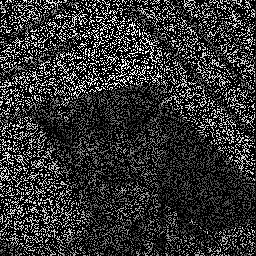
\includegraphics[width = 0.4\linewidth]{foreman_large_masked_43.png}
%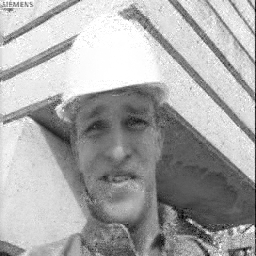
\includegraphics[width = 0.5\linewidth]{foreman_large_rec_42.png}
\end{minipage}
\begin{minipage}{0.8\linewidth}
\centering
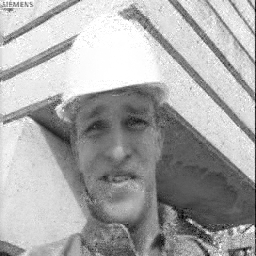
\includegraphics[width = 0.4\linewidth]{foreman_large_rec_42.png}
%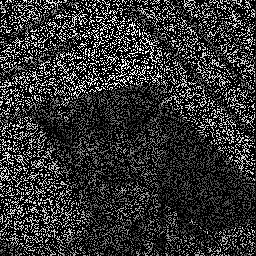
\includegraphics[width = .5\linewidth]{foreman_large_masked_43.png}
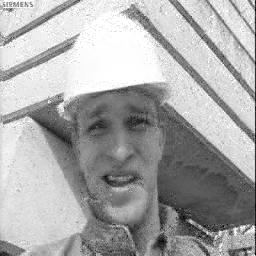
\includegraphics[width = 0.4\linewidth]{foreman_large_rec_43.png}
\scriptsize\hphantom{.}\hspace{2.5cm} frame 42 \hspace{3cm} frame 43
\end{minipage}\\
\begin{minipage}{0.95\linewidth}
\caption{Two consucutive frames of a sample video signal.
  Top row: The sensing mechanism $\bm\Theta$ has measured 30\% of the original samples in $\bm v$. 
  Bottom row: Recovered signal using a cascade of RVMs. The error is 6.9\%.}
\label{fig}
\end{minipage}
\end{figure}
In Figure \ref{fig}, the sensing mechanism $\bm\Theta$ corresponds to \emph{signal mask}.
For such $\bm\Theta$, the reconstruction quality can be boosted by building a cascade of RVMs \cite{pilikos2014}.


\end{block}
%\normalsize
%%%%%%%%%%%%%%%%%%%%%%%%%%%%%%%%%%%%%%%%%%%% References %%%%%%%%%%%%%%%%%%%%%%%%%%%%%%%%%%%%%%%%%%%%%%
\begin{block}{References and Acknowledgements}
\begin{minipage}{.9\linewidth}
     {     \printbibliography   % i.e. the references.bib file
     } 
\end{minipage}
\vspace{2ex}
% {
% \tiny Thanks to my sponsor, my supervisor, and to other students for
%   fruitful discussions and caffeine.
% \par
% }
\end{block}

\end{textblock}

\end{frame}
\end{document}
